\documentclass[usenames,dvipsnames]{beamer}
\usetheme{ensam}
\usepackage{pgfplots}
\usepackage{subcaption}
\usepackage{acronym}
\usepackage{pgfplots}
\usepackage{tikz}
\usetikzlibrary{calc, shapes, fit}
\usepackage{amsmath}
\usepackage{algorithmic}
\usepackage{mynotations}
\usepackage{algorithm}
\usepackage{eqparbox}
\usepackage[font=scriptsize]{caption}
\usetikzlibrary{bayesnet,positioning,calc}

\tikzstyle{obs} = [latent,fill=lightBlue]

\tikzstyle{default}=[draw=sexyRed,thick,rounded corners,text width=0.5in,font=\scriptsize,align=center]
\usepgfplotslibrary{colorbrewer}
\definecolor{ForestGreen}{RGB}{34,139,34}
\newcommand{\comment}[1]{\textcolor{ForestGreen}{#1}}
%algorithmic comment
\renewcommand\algorithmiccomment[1]{%
  \hfill\comment{\#\scriptsize\eqparbox{COMMENT}{#1}}%
}
\title{Applications}
\author{\underline{A.Belcaid}}
\institute{\small Université Euromed de Fès} 

%tikz bayesian theme
\usetikzlibrary{bayesnet,positioning,calc}
\tikzstyle{obs} = [latent,fill=lightBlue]
\tikzstyle{default}=[draw=sexyRed,thick,rounded corners,text width=0.5in,font=\scriptsize,align=center]
\DeclareMathOperator{\argmin}{argmin}

\pgfplotsset{every tick label/.append style={font=\tiny}}





% add bibliography

\begin{document}
\maketitle

\begin{frame}
\tableofcontents
\end{frame}
%{{{ Introduction 

% Définition {{{ %
\begin{frame}[<+->]
  \frametitle{Définition}
  \small
  \begin{block}{Définition}
    One appelle une \textbf{\alert{application}} $f: E\rightarrow F$ entre deux ensembles $E$ et
    $F$, une correspondance qui associe a \textbf{\structure{tout}} élément
    $ x \in E$ un élément \textbf{\alert{unique}} $y\in F$   noté $f(x)$
  \end{block}
 \begin{center}
 \begin{tikzpicture}[scale=1, transform shape]
   \node[ellipse, minimum width=1.5cm, minimum height=2.5cm, draw=sexyRed!80,
     thick, label=left:$E$] at(0,0)  {};
   \node[ellipse, minimum width=1.5cm, minimum height=2.5cm, draw=Apricot,
     thick, label=right:$F$] at(3,0)  {};
   \node[point, fill=sexyRed!80, label=left:$x$] (A) at (0.2,0.5){};
   \node[point, fill=sexyRed!80] (B) at (0.1,0.0){};
   \node[point, fill=sexyRed!80] (C) at (-0.15,-0.4){};

   \node[point, fill=Apricot,xshift=3cm, label=above right:$f(x)$] (fA) at (0.2,0.5){};
   \node[point, fill=Apricot,xshift=3cm] (fB) at (0.1,0.0){};
   \node[point, fill=Apricot,xshift=3cm] (fC) at (0.15,-0.6){};

   \path[->,>=stealth, thick] (A) edge[bend left=45] (fA);
   \path[->,>=stealth, thick] (B) edge[bend left=35] (fB);
   \path[->,>=stealth, thick] (C) edge[bend right=35] (fB);
 \end{tikzpicture}
 \end{center}
 \pause

 \begin{itemize}
   \item $E$: \textbf{Ensemble de départ}.
   \item $F$: \textbf{Ensemble d'arrivée}.
 \end{itemize}
\end{frame}


\begin{frame}[<+->]
  \frametitle{Application sur $\mathbb{R}$}
  \begin{itemize}
    \item Si $E$ et $F$ sont des \textbf{sous ensembles}  de $\R$. On peut
      représenter $f : \R\rightarrow\R$ par son \alert{\textbf{graphe}}:
      \begin{equation}
        \Gamma_f = \left\{ \big(x,f(x)\big)\in E\times F\;|\; x\in E \right\}
      \end{equation}
  \end{itemize} 
\pause

\begin{center}
\begin{tikzpicture}[yscale=0.8, transform shape]
  \draw[ ->, >=stealth ] (-2,0)--(5,0);
  \draw[ ->, >=stealth ] (0,-1)--(0,4);
  \node at (5,-0.2) {$x$};
  \node at (-0.2,5) {$y$};
  \draw[very thick, Apricot] (-1,0.5) ..controls (1.5, 2) and (2,.9).. (4.5, 1.5);
  \node[point, fill=sexyRed!80, label=below:$x$]  (X) at (1,0){};
  \node[point, fill=sexyRed!80, label=left:$y$]  (Y) at (0,1.3){};
  \node[point, fill=sexyRed!80,label=above:$f(x)$]  (A) at (1,1.3){};
  \node[label=above:$\Gamma_f$]  at (3,1.1){};
  \path[draw] (X)--(A)--(Y);
\end{tikzpicture}
\end{center}
\end{frame}


\begin{frame}[t]
  \frametitle{Égalité et Composition}
 \begin{block}{Égalité}
   Deux applications $f$ et $g: E\rightarrow F$ sont dites \textbf{\alert{égales}} $f=g$ si:
   \begin{equation*}
     \forall x \in E\quad f(x) = g(x)
   \end{equation*}
 \end{block} 
 \pause

 \begin{block}{Composition}
   Soit les deux applications $f: E\rightarrow F$ et $g:F\rightarrow G$. On
   définit alors la \textbf{\alert{composée}}:
   \begin{equation*}
     \left( g\circ f\right)(x) = g\left( f(x)\right)
   \end{equation*}
 \end{block}
 \pause
 \begin{center}
 \begin{tikzpicture}[scale=1,>=stealth]
   \node[] (E) at (0,0) {$E$};  
   \node[] (F) at (3,0) {$F$};  
   \node[] (G) at (6,0) {$G$};  
   \path[->, draw] (E)--(F);
   \path[->, draw] (F)--(G);

   \path[thick,->,>=stealth,draw, Apricot] (E)edge[bend left=35]node[pos=0.5, label=above:$f$]{}(F);
   \path[thick,->,>=stealth,draw,Apricot] (F)edge[bend left=35]node[pos=0.5, label=above:$g$]{}(G);

   \path[thick,->,>=stealth,draw,sexyRed] (E)edge[bend right=25]node[pos=0.5,
     label=below:$g\circ f$]{}(G);
 \end{tikzpicture}
 \end{center}
\end{frame}

\begin{frame}[t]
  \frametitle{Identité}
  \small
 \begin{block}{Identité}
   Une application particulière est l'application \textbf{\textbf{identité}}:
   \begin{eqnarray*}
     \text{id}_E &:& E\rightarrow E\\
                && x \rightarrow x
   \end{eqnarray*}
 \end{block} 
 \pause

 \begin{block}{Mini Exercice}
   Soit $f: ]0,+\infty[\rightarrow ]0,+\infty[$ tel que $f(x)=\dfrac{1}{x}$, et
   $g: ]0,+\infty[\rightarrow \R$  tel que $g(x) = \dfrac{x-1}{x+1}$.
   \begin{itemize}
     \item Donner $f\circ\text{id}$, $\text{id}\circ g$, $g\circ f$ et $f\circ
       g$.
   \end{itemize}
 \end{block}
\end{frame}
% }}} Définition %

%}}}
% Image directe, Image réciproque {{{ %
%{{{ Image directe
\begin{frame}[t]
  \frametitle{Image directe}

  \begin{block}{Image directe}
    Soit $f: E\rightarrow F$ une application, et $\mathbf{A}$ une partie de $E$.
    On note l'\alert{\textbf{image directe}} de $A$ par $f$ l'ensemble:
    
    \begin{equation}
      f(A) = \left\{ f(x)\;|\; x\in E\right\}
    \end{equation}
  \end{block}
  \begin{columns}
    \begin{column}{0.5\textwidth}
      \begin{center}   
        \begin{tikzpicture}
   \node[ellipse, minimum width=1.5cm, minimum height=2.5cm, draw,
     thick, label=left:$E$] at(0,0)  {};
   \node[ellipse, minimum width=1.5cm, minimum height=2.5cm, draw,
     thick, label=right:$F$] at(3,0)  {};
   \node[point, fill=sexyRed!80] (A) at (0.2,0.5){};
   \node[point, fill=sexyRed!80] (B) at (0.1,0.0){};
   \node[point, fill=sexyRed!80] (C) at (-0.15,-0.4){};

   \node[point, fill=Apricot,xshift=3cm ] (fA) at (0.2,0.5){};
   \node[point, fill=Apricot,xshift=3cm] (fB) at (0.1,0.0){};
   \node[point, fill=Apricot,xshift=3cm] (fC) at (0.15,-0.6){};

   \path[->,>=stealth, thick] (A) edge[bend left=45] (fA);
   \path[->,>=stealth, thick] (B) edge[bend left=35] (fB);
   \path[->,>=stealth, thick] (C) edge[bend right=35] (fB);
   \node[draw=Apricot, thick, fit=(A)(B), rounded corners,label=left:$A$]{};
   \node[draw=sexyRed, thick, fit=(fA)(fB), rounded corners]{};
   \node at (3,1){\tiny$f(A)$};
 \end{tikzpicture}
 \end{center}
    \end{column}
    \begin{column}{0.5\textwidth}
      \begin{center}      
        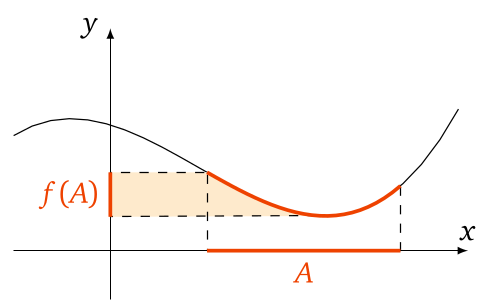
\includegraphics[width=4.5cm, height=3.5cm]{./image_directe.png}
\end{center}
    \end{column}
  \end{columns}
\end{frame}
%}}}
% Image réciproque {{{ %
\begin{frame}[t]
  \frametitle{Image Réciproque}

  \begin{block}{Image directe}
    Soit $B\subset F$ et $f:E\rightarrow F$ une application de $E$ dans $F$. On
    définit \textbf{\alert{l'image réciproque}} de $B$ par f: 
    
    \begin{equation}
      f^{-1}(B) = \left\{ x \in A\;|\; f(x)\in B\right\}
    \end{equation}
  \end{block}
  \begin{columns}
    \begin{column}{0.5\textwidth}
      \begin{center}   
        \begin{tikzpicture}
   \node[ellipse, minimum width=1.5cm, minimum height=2.5cm, draw,
     thick, label=left:$E$] at(0,0)  {};
   \node[ellipse, minimum width=1.5cm, minimum height=2.5cm, draw,
     thick, label=right:$F$] at(3,0)  {};
   \node[point, fill=sexyRed!80] (A) at (0.2,0.5){};
   \node[point, fill=sexyRed!80] (B) at (0.1,0.0){};
   \node[point, fill=sexyRed!80] (C) at (-0.15,-0.4){};

   \node[point, fill=Apricot,xshift=3cm ] (fA) at (0.2,0.5){};
   \node[point, fill=Apricot,xshift=3cm] (fB) at (0.1,0.0){};
   \node[point, fill=Apricot,xshift=3cm] (fC) at (0.15,-0.6){};

   \path[->,>=stealth, thick] (A) edge[bend left=45] (fA);
   \path[->,>=stealth, thick] (B) edge[bend left=35] (fB);
   \path[->,>=stealth, thick] (C) edge[bend right=35] (fB);
   \node[draw=Apricot, thick, fit=(fB)(fC), rounded corners,label=right:$B$]{};
   \node[draw=sexyRed, thick, fit=(B)(C), rounded corners]{};
   \node at (0,-0.8){\scriptsize$f^{-1}(B)$};
 \end{tikzpicture}
 \end{center}
    \end{column}
    \begin{column}{0.5\textwidth}
      \begin{center}      
        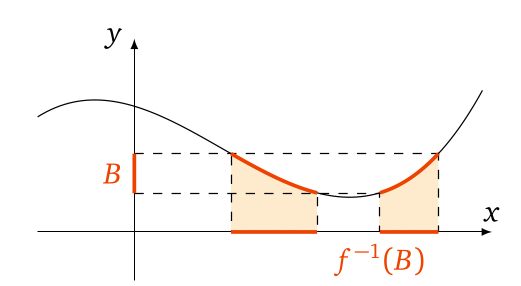
\includegraphics[width=4.5cm, height=3.5cm]{./image_reciproque.png}
\end{center}
    \end{column}
  \end{columns}
\end{frame}
% }}} Image réciproque %

% Antécédants {{{ %
\begin{frame}[t]
  \frametitle{Antécédents}
  
  \begin{block}{Antécédent}
    Soit une application $f:E\rightarrow F$ et $y\in F$. Un élément $\mathbf{x}$
    est un \textbf{\alert{antécédent}} de $y$ si on as 
    \begin{equation*}
      y = f(x)
    \end{equation*}
  \end{block}
  \begin{columns}
    \begin{column}{0.5\textwidth}
      \begin{center}   
        \begin{tikzpicture}
   \node[ellipse, minimum width=1.5cm, minimum height=2.5cm, draw,
     thick, label=left:$E$] at(0,0)  {};
   \node[ellipse, minimum width=1.5cm, minimum height=2.5cm, draw,
     thick, label=right:$F$] at(3,0)  {};
   \node[point] (A) at (0.2,0.5){};
   \node[point, fill=sexyRed!80,label=left:$x_1$] (B) at (0.1,0.0){};
   \node[point, fill=sexyRed!80,label=left:$x_2$] (C) at (-0.15,-0.4){};
   \node[point, fill=sexyRed!80,label=left:$x_3$] (D) at (-0,-0.7){};

   \node[point, fill=Apricot,xshift=3cm ] (fA) at (0.2,0.5){};
   \node[point, fill=Apricot,xshift=3cm, label=right:$y$] (fB) at (0.1,0.0){};
   \node[point, fill=Apricot,xshift=3cm] (fC) at (0.15,-0.6){};

   \path[->,>=stealth, thick] (A) edge[bend left=45] (fA);
   \path[->,>=stealth, thick] (B) edge[bend left=35] (fB);
   \path[->,>=stealth, thick] (C) edge[bend right=35] (fB);
   \path[->,>=stealth, thick] (D) edge[bend right=35] (fB);
 \end{tikzpicture}
 \end{center}
    \end{column}
    \begin{column}{0.5\textwidth}
      \begin{center}      
        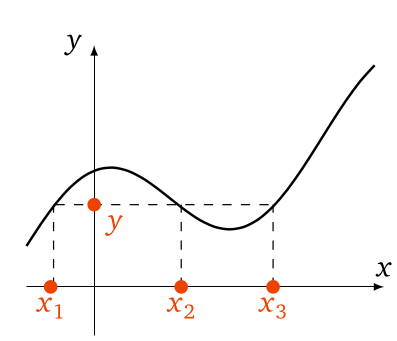
\includegraphics[width=4.5cm, height=3.5cm]{./antecedent.png}
\end{center}
    \end{column}
  \end{columns}
\end{frame}
% }}} Antécédants %
% Mini exercices {{{ %
\begin{frame}[<+->]
  \frametitle{Mini exercices}
  \small
  \begin{itemize}
    \item Soient $f$ et $g: E\rightarrow F$ deux applications. Donner la
      \textbf{négation}   de $f=g$.
    \item Représenter le graphe de la fonction $f:\N\rightarrow\R$ définie par
      $f(n)=\dfrac{4}{n+1}$
    \item Soient $f, g$ et $h: \R\rightarrow\R$ définies par:
      \begin{itemize}
        \item $f(x) = x^2$
        \item $g(x) = 2x + 1$
        \item $h(x) = x^3 - 1$
      \end{itemize}
      Donner l'expression des fonctions suivantes: $f\circ\left(h\circ h\right)$ et
      $\left(f\circ g\right)\circ h$
      \item Soit la fonction $f:\R\rightarrow\R$ définie par $f(x)=x^2$. Donner
        les ensembles suivants: $f([0,1[)$, $f(\R)$, $f(]-1,2[)$,
        $f^{-1}([1,2[)$, $f^{-1}(]-1,1[)$, $f^{-1}(3)$.
  \end{itemize}
\end{frame}
% }}} Mini exercices %


% }}} Image directe, Image réciproque %
% Antécedants {{{ %
% }}} Antécedants %
%}}}
% Injection / Surjection / Bijection {{{ %

% Injection {{{ %
\begin{frame}[<+->]
  \frametitle{Injection/Surjection/Bijection}
  \begin{block}{Définition}
  Soit $E$ et $F$ deux ensembles et $f:E\rightarrow F$ une application.
  L'application $f$ est dite \textbf{\alert{injective}} si:

  \begin{equation}
    \forall x_1,x_2 \in E\quad \big(  f(x_1) = f(x_2) \implies x_1= x_2\big)
  \end{equation}


\end{block}  

      \begin{center}   
        \begin{tikzpicture}
   \node[ellipse, minimum width=1.5cm, minimum height=2.5cm, draw,
     thick, label=left:$E$] at(0,0)  {};
   \node[ellipse, minimum width=1.5cm, minimum height=2.5cm, draw,
     thick, label=right:$F$] at(3,0)  {};
   \node[point] (A) at (0.2,0.5){};
   \node[point] (B) at (0.1,0.0){};
   \node[point] (C) at (-0.15,-0.4){};

   \node[point, fill=Apricot,xshift=3cm ] (fA) at (0.2,0.5){};
   \node[point, fill=Apricot,xshift=3cm] (fB) at (0.1,0.0){};
   \node[point, fill=Apricot,xshift=3cm] (fC) at (0.15,-0.6){};
   \node[point, fill=Apricot,xshift=3cm] (fD) at (0,-0.8){};

   \path[->,>=stealth, thick] (A) edge[bend left=45] (fA);
   \path[->,>=stealth, thick] (B) edge[bend left=35] (fB);
   \path[->,>=stealth, thick] (C) edge[bend left=25] (fC);
 \end{tikzpicture}
 \end{center}

  \begin{itemize}
    \small
  \item Formuler l'injectivité en utilisant la notion
    d'\textbf{\alert{antécedent}}?
  \end{itemize}
\end{frame}
% }}} Injection %
% Surjection {{{ %

\begin{frame}[<+->]
  \frametitle{Surjection}
  \begin{block}{Définition}
  Soit $E$ et $F$ deux ensembles et $f:E\rightarrow F$ une application.
  L'application $f$ est dite \textbf{\alert{surjective}} si:

  \begin{equation}
    \forall y \in F\quad \exists x\in E   \left(y = f(x)\right)
  \end{equation}


\end{block}  


\begin{columns}
  \begin{column}{0.5\textwidth}
    
      \begin{center}   
        \begin{tikzpicture}
   \node[ellipse, minimum width=1.5cm, minimum height=2.5cm, draw,
     thick, label=left:$E$] at(0,0)  {};
   \node[ellipse, minimum width=1.5cm, minimum height=2.5cm, draw,
     thick, label=right:$F$] at(3,0)  {};
   \node[point] (A) at (0.2,0.5){};
   \node[point] (B) at (0.1,0.0){};
   \node[point] (C) at (-0.15,-0.4){};
   \node[point ] (D) at (0,-0.8){};

   \node[point, fill=Apricot,xshift=3cm ] (fA) at (0.2,0.5){};
   \node[point, fill=Apricot,xshift=3cm] (fB) at (0.1,0.0){};
   \node[point, fill=Apricot,xshift=3cm] (fC) at (0.15,-0.6){};

   \path[->,>=stealth, thick] (A) edge[bend left=45] (fA);
   \path[->,>=stealth, thick] (B) edge[bend left=35] (fB);
   \path[->,>=stealth, thick] (C) edge[bend left=25] (fC);
   \path[->,>=stealth, thick] (D) edge[bend left=25] (fC);
 \end{tikzpicture}
 \end{center}
  \end{column}
  \begin{column}{0.5\textwidth}
   \begin{center}
     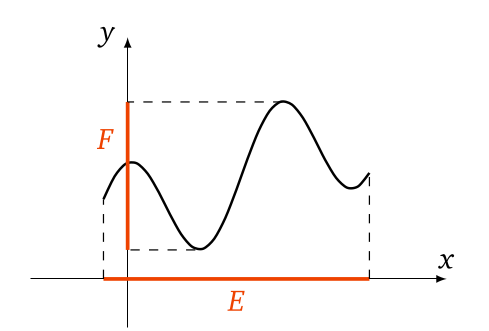
\includegraphics[width=4.5cm, height=3.5cm]{./surjection.png}
   \end{center} 
  \end{column}
\end{columns}

  \begin{itemize}
    \small
  \item Formuler la surjectivitié en utilisant la notion
    d'\textbf{\alert{antécedent}}?
  \end{itemize}

\end{frame}


\begin{frame}[<+->]
  \frametitle{Tester vos connaissances}

  \begin{columns}
    \begin{column}{0.5\textwidth}
      \only<1->{

        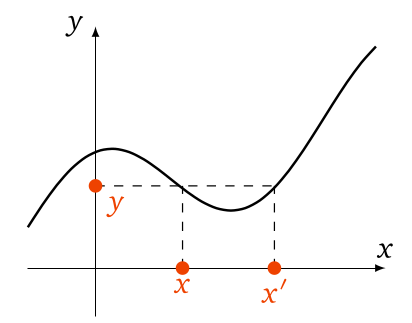
\includegraphics[width=4cm, height=4cm]{./injectivit_q1.png}
      } 

      \only<2->
      {

        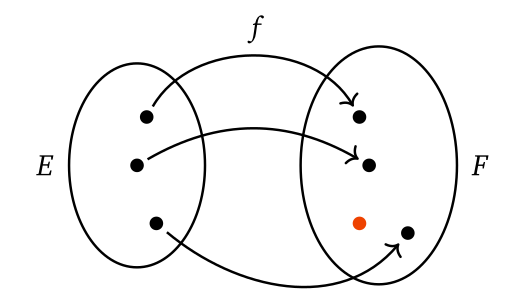
\includegraphics[width=4cm, height=4cm]{./injectivit_q2.png}
      }
    \end{column}
    \begin{column}{0.5\textwidth}
      
      \only<3->
      {

        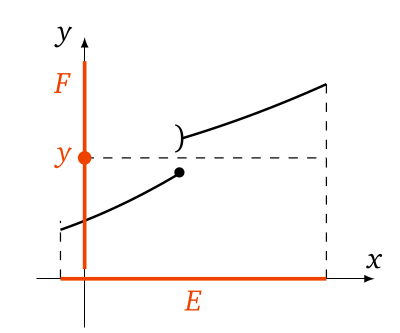
\includegraphics[width=4cm, height=4cm]{./injectivit_q3.png}
      }

      \only<4->
      {

        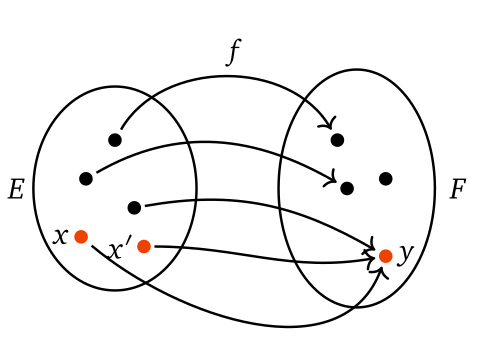
\includegraphics[width=4cm, height=4cm]{./injectivit_q4.png}
      }
    \end{column}
  \end{columns}
  
\end{frame}


\begin{frame}[t]
  \frametitle{Exercices rapides}
 \begin{block}{Exemple 1}
   Domontrer que la fonction $f: \N\rightarrow \Q$ définie par $f(n) =
   \dfrac{1}{n+1}$ est \textbf{injective}. 
 \end{block} 
 \begin{block}{Exemple 2}
   Démonter par \textbf{\alert{contre exemple}}  que la fonction $x^3$ n'est pas
   \textbf{injective}.
 \end{block}

 \begin{block}{Exemple 3}
   
   La fonction $g:\R\rightarrow\R$ est elle \textbf{\alert{surjective}}?
 \end{block}
\end{frame}
% }}} Surjection %
% Bijection {{{ %
\begin{frame}[t]
  \frametitle{Injectivité}
 \begin{block}{Définition}
   Une fonction $f:E\rightarrow F$ est dite \textbf{\alert{bijective}} si elle est injective et
   surjective. Cela revient à dire que:

   \begin{equation}
     \forall y\in F\quad \alert{\exists!} x \in E \quad \left( y = f(x)\right)
   \end{equation}
 \end{block} 

 \begin{columns}
   \begin{column}{0.5\textwidth}

      \begin{center}   
        \begin{tikzpicture}
   \node[ellipse, minimum width=1.5cm, minimum height=2.5cm, draw,
     thick, label=left:$E$] at(0,0)  {};
   \node[ellipse, minimum width=1.5cm, minimum height=2.5cm, draw,
     thick, label=right:$F$] at(3,0)  {};
   \node[point] (A) at (0.2,0.5){};
   \node[point] (B) at (0.1,0.0){};
   \node[point] (C) at (-0.15,-0.4){};

   \node[point, fill=Apricot,xshift=3cm ] (fA) at (0.2,0.5){};
   \node[point, fill=Apricot,xshift=3cm] (fB) at (0.1,0.0){};
   \node[point, fill=Apricot,xshift=3cm] (fC) at (0.15,-0.6){};

   \path[->,>=stealth, thick] (A) edge[bend left=45] (fA);
   \path[->,>=stealth, thick] (B) edge[bend left=35] (fB);
   \path[->,>=stealth, thick] (C) edge[bend left=25] (fC);
 \end{tikzpicture}
 \end{center}
     
   \end{column}
   \begin{column}{0.5\textwidth}
     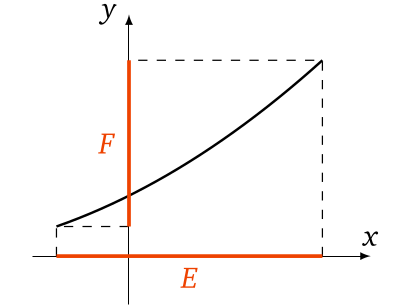
\includegraphics[width=4cm, height=4cm]{./bijective.png}  
   \end{column}
 \end{columns}
\end{frame}

\begin{frame}[t]
  \frametitle{Résultat Bijection}
  \normalsize
  \begin{block}{Proposition}
    Soit $E$, $F$ deux ensembles et $f: E\rightarrow F$ une application.

    \begin{enumerate}
      \item L'application $f$ est bijective si et seulement si il existe une
        application $g:F\rightarrow E$ telle que:
        \begin{itemize}
          \item $f\circ g=\text{id}_F$ 
          \item  $g\circ f = \text{id}_E$.
        \end{itemize}
      \item Si $f$ est bijective alors l'application $g$ est
        \textbf{\alert{unique}}  et elle est aussi bijective.
    \end{enumerate}
 \end{block}  

 \begin{itemize}
   \item L'applicaiton $g$ s'appelle \textbf{\alert{bijection réciproque}} de
     $f$ est elle est notée $f^{-1}$. On vérifie que $(f^{-1})^{-1}= f$
 \end{itemize}
 \begin{block}{Exemple}
   La bijection réciproque de la fonction 
   $f:R\rightarrow ]0,\infty[$ par $f(x)= \exp(x)$
  est la fonction $g: ]0,\infty[ \rightarrow \R$ par $g(x)=ln(x)$
 \end{block}
\end{frame}

\begin{frame}[t]
  \frametitle{Résultat Bijection}

  \begin{block}{Proposotion}
 Soit $f: E\rightarrow F$ et $ g:F\rightarrow G$ deux applications.
 \begin{itemize}
   \item Si les deux applications $f$ et $g$ sont injectives, alors $g\circ f$
     est injective.   

   \item Si les deux applications $f$ et $g$ sont surjectives, alors $g\circ f$
     est surjective.   
   \item  Ainsi si, $f$ et $g$ sont bijectives, alors $g\circ f$ est bijective.
 \end{itemize}

  \end{block}


 Alors l'application $(g\circ f)$ est \textbf{\alert{bijective}}. Sa bijection
 réciproque est donnée par:
 \begin{equation}
   \left(g\circ f\right)^{-1} = f^{-1}\circ g^{-1}
 \end{equation}
\end{frame}

  \begin{frame}[t]
    \frametitle{Mini Exercices}
    \begin{itemize}
      \item Les fonctions suivantes sont-elles injectives, surjectives,
        bijectives?

        \begin{enumerate}
          \item $f_1: \R\rightarrow [0,\infty[$, $f_1(x)=x^2$.\\[6pt]
          \item $f_2: [0,\infty]\rightarrow [0,\infty[$, $f_2(x)=x^2$.\\[6pt]
          \item $f_3: \N\rightarrow \N$, $f_3(n)=n^2$.\\[6pt]
          \item $f_4: \Z\rightarrow \Z$, $f_4(n)=n-7$.\\[6pt]
          \item $f_5: \R\rightarrow [0,\infty]$, $f_5(x)=\vert x\vert$.\\[6pt]
        \end{enumerate}
      \item Montrer que la fonction $f:]1,\infty[ \rightarrow ]0,\infty[$
        définie par $f(x)= \dfrac{1}{x-1}$ est bijective. Calculer sa bijection
        réciproque.
    \end{itemize} 
  \end{frame}
% }}} Bijection %

% }}} Injection / Surjection / Bijection %
% Ensemble finies {{{ %
% Cardinal {{{ %
%{{{ Définition cardinal
\begin{frame}[<+->]
  \frametitle{Ensembles finis}
  \begin{block}{Cardinal}
    Un ensemble $E$ est \textbf{\alert{fini}} si il existe une bijection entre
    $E$ et l'ensemble $\{1,2,\ldots, n\}$.\\[4pt]

    Dans ce cas l'entier $n$ s'appelle \alert{\textbf{cardinal}} de $E$ et il est
    noté $\Card E$ ou $\vert E\vert$.
  \end{block}
  
  Voici quelque exemples:
  \begin{enumerate}
    \item $E = \{\text{Rouge}, \text{Bleu}, \text{Vert}\}$ est de $\Card
      E=3$.\\[4pt]
    \item $\N$ n'est pas un ensemble fini.\\[4pt]
    \item Le cardinal de $\emptyset$ est $0$.\\[4pt]
  \end{enumerate}
\end{frame}
%}}}
% Propriétées  {{{ %
\begin{frame}[<+->]
  \frametitle{Propriétés Cardinal}
 \begin{block}{Propriétés Cardinal}
   \begin{itemize}
     \item Si $B\subset A$ et $A$ est \textbf{fini}. Alors $B$ est aussi fini et 
       \begin{equation}
         \Card B \leq \Card A
       \end{equation}
      \begin{equation}
        \Card (A-B) =\Card A - \Card B
      \end{equation}
      Ainsi si $\Card A = \Card B  \implies A = B$\\[8pt]
    \item Pour deux ensembles $A$ et $B$ \textbf{\alert{disjoints}}:
      \begin{equation}
        \Card(A\cup B) = \Card A + \Card B
      \end{equation}
  \end{itemize} 
 \end{block} 
\end{frame}
% }}} Propriétées  %
% Cardinal Union {{{ %
\begin{frame}[t]
  \frametitle{Cardinal union}
 \begin{block}{Cardinal Union}
      Pour deux ensembles quelconques
      \begin{equation}
        \Card(A\cup B) = \Card A + \Card B - \Card(A\cap B)
      \end{equation}
 \end{block} 
 \vspace*{1cm}
\begin{center}
 \begin{tikzpicture}[scale=0.7, transform shape]
   \node[ellipse,draw=sexyRed, minimum width=3cm, minimum height=4cm, thick,
   rotate=45, label=left:$E$] at (0,0) (E){};
   \node[xshift=1.5cm, ellipse,draw=Apricot, minimum width=3cm, minimum
   height=3cm, thick, label=right:$F$] at (0,0) (E){};
   \node[point, xshift=-0.5cm] (A) at (0,0){};
   \node[point, xshift=-0.5cm] (A) at (0,-1.2){};
   \node[point, xshift=-0.5cm] (A) at (-1,1.0){};
   \node[point, xshift=-0.5cm] (A) at (0,1){};
   \node[point, xshift=-0.5cm] (A) at (1,0.8){};
   \node[point, xshift=-0.5cm] (A) at (1,0){};
   \node[point, xshift=-0.5cm] (A) at (1.2,0.5){};
   \node[point, xshift=-0.5cm] (A) at (2,1){};
   \node[point, xshift=-0.5cm] (A) at (3,0){};
 \end{tikzpicture}
 \end{center}
 \begin{itemize}
   \item \textbf{\alert{Preuve:}} Utiliser la décomposition:
     \begin{equation*}
       A\cup B = A \cup \left(B - \left(A\cap B\right)\right)
     \end{equation*}
 \end{itemize}
\end{frame}
% }}} Cardinal Union %
% }}} Cardinal %
% Relation avec l'injectivité {{{ %

% Relation Injectivité {{{ %
\begin{frame}[t]
  \frametitle{Relation avec Injectivité, Surjectivité}
 \begin{block}{Proposition}
   Soit $E$ et $F$ deux ensembles finis et $f:E\rightarrow F$ une application.
   Alors:

   \begin{enumerate}
     \item Si $f$ est \alert{injective} alors $\Card E \leq \Card F$.\\[8pt]
     \item Si $f$ est \alert{surjective} alors $\Card E \geq \Card F$.\\[8pt]
     \item Si $f$ est \alert{bijective} alors $\Card E = \Card F$.\\[8pt]
   \end{enumerate}
 \end{block} 
 \pause
 \begin{block}{Démonstration}
   \begin{itemize}
     \scriptsize
     \item Supposons que $f$ est injective. Notons $F^{'}=f(E)\subset F$ l'image directe
       de $E$. Ainsi  chaque élément de $F^{'}$ admet un antécédent unique
       dans $E$. On conclut que $\Card F^{'} = \Card E \leq \Card F$.
     \item Supposons que $f$ est surjective, Ainsi tous les éléments de $F$
       admet au moins un antécédent, On conclut alors que $\Card E \geq \Card
       F$.
   \end{itemize} 
 \end{block}
\end{frame}
% }}} Relation Injectivité %

% Equivalence {{{ %
\begin{frame}[t]
  \frametitle{ Egalité cardinal}
 \begin{block}{Proposition}
  Soit $E$ et $F$ deux ensembles et $f:E\rightarrow F$ une application. Si 
  \begin{equation}
    \Card E = \Card F
  \end{equation}
  les trois propriétés suivantes sont équivalentes:
  \begin{enumerate}
    \item $f$ est injective.\\[8pt]
    \item $f$ est surjective.\\[8pt]
    \item $f$ est bijective.\\[8pt]
  \end{enumerate}
 \end{block} 
 \begin{itemize}
   \item \alert{\textbf{Indice:}} Prouver que $(1)\implies (2)\implies
     (3)\implies (1) $
 \end{itemize}
\end{frame}
% }}}  Equivalence %

% }}} Relation avec l'injectivité %
% Nombre d'applications {{{ %
% Nombre d'applications {{{ %
\begin{frame}[t]
  \frametitle{Nombre d'applications}
 \begin{block}{Proposition}
   Soit $E$ et $F$ tel que $\Card E = n$ et $\Card F=p$.\\[8pt]

   Alors le nombre d'applications \emph{différentes} entre $E$ et $F$ est
   $\mathbf{p^n}$
 \end{block} 
 \begin{itemize}
   \item \textbf{\alert{Indice Preuve:}} On fixe l'ensemble $F$ et on démontre
     par récurrence sur le cardinal de $E$.
 \end{itemize}
 \begin{block}{Exemple}
   \begin{itemize}
     \item Donner le nombre d'application entre $\{0,1,3\}$ et $\{0,1,2\}$.
     \item \textbf{Codage binaire}: Combien de nombre entiers peut on
       \textbf{\alert{coder}} sur $8$ bits. 
   \end{itemize}
 \end{block}
\end{frame}

\begin{frame}[<+->]
  \frametitle{Nombre d'injections}
 
  \begin{block}{Nombre d'injections}
   Soit $E$ et $F$ tel que $\Card E= n$ et $\Card F=p$. Alors le nombre
   \textbf{d'injections} est donné par:

   \begin{equation*}
     p\times (p-1) \times (p-2)\times \ldots \times\left(p-(n-1)\right)
   \end{equation*}
  \end{block}

  \begin{itemize}
    \item \alert{\textbf{Indice Preuve:}} Fixer l'ensemble $F$ et considérer une
      récurrence sur $E$.
  \end{itemize}
  \pause
  \begin{block}{Bijections}
   Le nombre de bijections entre deux ensembles de même cardinal est $n$ :

   \begin{equation*}
     n!
   \end{equation*}
  \end{block}
\end{frame}
% }}} Nombre d'applications %
% Nombre sous ensembles {{{ %

\begin{frame}[t]
  \frametitle{Nombre sous ensembles}
 \begin{block}{Nombre sous ensemble}
   Soit $E$ un ensemble fini tel que $\Card E = n$. 
   Le nombre de sous ensembles de $E$  est donné par:
   \begin{equation}
     \Card \mathcal{P}(E) = 2^n
   \end{equation}
 \end{block} 
 \pause
 \begin{block}{Exemple}
   Énumérer les éléments de $\mathcal{P}\big( \{1,2,3,4,5\}\big)$ selon leur
   cardinal.
 \end{block}
 \begin{itemize}
   \item \textbf{\alert{Indice preuve:}}: Utiliser une récurrence sur le
     cardinal de $E$.
 \end{itemize}
\end{frame}

% }}} Nombre sous ensembles %
% Coefficients de Binome {{{ %

% Coefficients de Binome {{{ %
\begin{frame}[t]
  \frametitle{Coefficients de Binôme}
  \begin{block}{Définition}
  Le nombre de parties contenant $\mathbf{k}$ éléments d'un ensemble de cardinal
  $n$ est noté $\mathbf{\binom{n}{k}}$ ou $C^{n}_{k}$.
  \end{block}
  \pause
  \begin{block}{Corrolaire}
    \begin{itemize}
      \item $\binom{n}{0} = 1$\\[8pt]\pause
      \item $\binom{n}{n} = 1$\\[8pt]\pause
      \item $\binom{n}{1} = n$\\[8pt]\pause
      \item $\binom{n}{k} = \binom{n}{n-k}$\\[8pt]\pause
      \item $\binom{n}{0}+\binom{n}{1}+\binom{n}{2}+\ldots \binom{n}{n}=2^n$.\pause
    \end{itemize}
  \end{block}
\end{frame}
% }}} Coefficients de Binome %

% Propriétées Binom {{{ %
\begin{frame}[<+->]
  \frametitle{Propriétées Coefficiens Binôme}
 \begin{block}{Proposition}

  \begin{equation}
    \binom{n}{k} = \binom{n-1}{k} + \binom{n-1}{k-1} \quad (0< k < n)
  \end{equation}
 \end{block} 

 \begin{itemize}
 \item \textbf{\alert{Indice preuve}}: Pour un un ensemble $E$ de cardinal
     $n$. Considérer un élément $x\in E$, Diviser les parties de taille $k$ en
     ceux qui contiennent $x$ et ce ceux qui ne le contiennent pas. 
 \end{itemize}
\end{frame}
% }}} Propriétées Binom %

% Proposition 2 {{{ %
\begin{frame}[<+->]
  \frametitle{Expression Coefficient Newton}
\begin{block}{Proposition}
  \begin{equation}
    \binom{n}{k} =  \dfrac{n!}{k!(n-k)!}
  \end{equation}
\end{block}
\pause

\begin{itemize}
  \item \alert{\textbf{Indice Preuve:}} Utiliser une récurrence sur $n$
    et la proposition précédante du cours.
\end{itemize}
\end{frame}

\begin{frame}[<+->]
  \frametitle{Mini exercices}
 \begin{enumerate}
   \small
   \item Donner le nombre d'injections entre un ensemble de cardina
     $\mathbf{n}$ et un autre de cardinal $n+1$.\\[8pt]
   \item Calculer le nombre main  de taille $5$ cartes d'un jeu de $32$
     cartes.\\[8pt]
   \item Calculer le nombre de listes de taille $3$ qu'on peut construire
     avec des chiffres ($<10$). Par exemple $(1,2,3)$ et $(2,2,3)$ mais
     pas $(10,2,3)$.\\[8pt]
 \end{enumerate} 

\end{frame}
% }}} Proposition 2 %
% }}} Coefficients de Binome %
% Formule de Newton {{{ %
% }}} Formule de Newton %


% }}} Ensemble finies %
\end{document}
